% !TEX root = /home/jd18380/Documents/compass_yr1/Mini_Project/Report/main.tex
\documentclass[a4paper]{article}

%% Language and font encodings
\usepackage[english]{babel}
\usepackage[utf8x]{inputenc}

\usepackage{booktabs}
\usepackage{tabu}
\usepackage[T1]{fontenc}
% \usepackage{subfig}
\usepackage{subcaption}
\usepackage{placeins}
\usepackage{multirow}

%% Sets page size and margins
\usepackage[a4paper,top=2cm,bottom=3cm,left=2cm,right=2cm,marginparwidth=2.75cm]{geometry}
%% Useful packages
\usepackage{amsmath}
\usepackage{amsfonts}
\usepackage{amssymb}
\usepackage{bm}
\usepackage{xcolor}
\DeclareMathOperator*{\argmax}{arg\!\max}
\DeclareMathOperator*{\argmin}{arg\!\min}
\usepackage[toc,page]{appendix}
\usepackage{graphicx}
%\usepackage{apacite}
\usepackage[colorinlistoftodos]{todonotes}
\usepackage[colorlinks=true, allcolors=blue]{hyperref}
\usepackage{cleveref}

\newtheorem{theorem}{Theorem}[section]
\newtheorem{corollary}{Corollary}[theorem]
\newtheorem{lemma}[theorem]{Lemma}
\newtheorem{definition}{Definition}[section]
\newtheorem{question}{Question}[section]

\title{Investigating the Effect of Latent Representations on Continual Learning Performance}
\author{By Henry Bourne, Supervised by Rihuan Ke}
\date{}

\begin{document}
\maketitle


\begin{abstract}
    In this report we demonstrate how neural networks trained on tasks sequentially forget how to perform previous tasks they've trained on when training on new tasks. We demonstrate forgetting on the split-MNIST using simple networks and then on split-CIFAR10 with networks composed of a pretrained encoder and a fully connected classifier on the end where the encoders were trained using different techniques. We found that using frozen latent representations or trainable latent representations had no effect on the forgetting rate of the network, however, trainable latent representations tended to be able to achieve a higher accuracy on the task currently being trained. We also found all our networks except the largest, trained on the largest pretraining dataset with a frozen latent representation had immediate complete forgetting of the previous task after one epoch of training on a new task. We also propose an extremely simple continual learning technique based on our findings.  
\end{abstract}

\section{Introduction}
In this report we investigate the effect of latent representations on continual learning performance. Continual learning \cite{de2021continual, parisi2019continual} describes a challenge were we try and train models on a series of tasks that are presented to the network in a sequential fashion, we are specifically concerned with the subset of continual learning where neural network architectures are the models being trained. We will also be mainly concerned with the problem of continually learning an image classification task. Usually these tasks contain very different data such as distinct classes and this means the assumption that our data is independently identically distributed, which we need to perform minibatch stochastic gradient descent, is broken. This leads to the problem of catastrophic forgetting \cite{ratcliff1990catastrophic, mccloskey1989catastrophic, french1999catastrophic} where a neural network will forget to correctly classify data from a previous task whilst learning on a new task, which means after sequentially learning a series of tasks the network will only be able to correctly classify images (with good performance) that are similar to data presented in the last task. 

We aimed through empirical analysis to investigate how using fixed latent representations might affect the degree to which a network forgets and also how we learnt the latent representation and what we learned it from might affect the degree of forgetting. We first demonstrated the problem of forgetting using simple networks, a fully connected network and a small convolutional neural network \cite{lecun1995convolutional}, on a simple continual learning dataset the MNIST handwritten digits dataset \cite{deng2012mnist} partitioned into 5 tasks where each task contains all the data corresponding to two classes (two digits). We found that the networks immediately forgot all knowledge on the previous task as soon as they started training on a new task. 

We then carried out experiments using Resnet18, VGG16 and autoencoder networks as encoders with some fully connected layers on the end for classification. These networks are all of varying sizes and had either no pretraining or were trained on CIFAR100 or Imagenet. For each network we also had two variations: one where the encoder was frozen and one where the encoder was trainable. We found that by the end of training on any task the previous task had been completely forgotten, ie. achieves an accuracy of zero or near zero on the previous task. Furthermore, we found that bar the network with frozen Resnet18 as the encoder every network immediately forgot all knowledge on the previous task (ie. achieving a training and testing accuracy of zero or very near zero) after just one epoch of training on the next task. This severe forgetting is somewhat surprising given the lesser extent of forgetting that has been shown in other papers such as in \cite{ramasesh2022effect,toneva2018empirical}, however, our increased number of tasks, smaller networks and not conducting interleaved training could explain our more severe results. Our results more closely resemble the kind of forgetting shown in \cite{mccloskey1989catastrophic}, however, the networks and datasets used to obtain the results are extremely simple. 

Our results from the network with frozen Resnet18 as the encoder showed some more gradual forgetting on some tasks. In \cite{ramasesh2022effect} the authors found that larger networks and larger pre-training datasets led to reduced forgetting which our results compliment as Resnet18 is the largest network that we experimented with, used the largest pretraining dataset we used (Imagenet) and was the only network to show more gradual forgetting. However, this doesn't explain why the non-frozen version of this network didn't also demonstrate slightly more gradual forgetting. This could suggest further avenues of exploration including conducting experiments on split-CIFAR10 with 5 tasks using larger networks with larger pre-training datasets and like we have done in this report comparing the amount of forgetting that occurs when we use a frozen encoder versus a non-frozen encoder. Our result with the frozen Resnet18 hints at the possibility that frozen representations might somewhat mitigate forgetting, which would run in opposition to what was found in \cite{ramasesh2020anatomy} where they found that almost all forgetting happens in the deepest layers but may agree with the work in \cite{rebuffi2017icarl} and \cite{li2017learning} where it appears that when training on tasks sequentially the encoder was mainly changed and not the classifier layers. An initial investigation into using larger networks showed even more gradual forgetting when the encoder was frozen (but not when the encoder was not trainable), suggesting there may be benefit to using fixed latent representations to hamper forgetting, further more rigorous investigation is of course required. However, we observed no changing in forgetting in any of the other networks when freezing the encoder which somewhat gives support to the findings in \cite{ramasesh2020anatomy}, that all or most forgetting happens in the deepest layers.

We also experimented with randomly initializing the fully connected, classifier, portions of the network at the end of each task and demonstrated that our results for the large part resembled the results without resetting the classifier. This is due to the fact that complete forgetting (accuracy on previously trained tasks is zero or near zero) is so immediate and that with a randomly initialized classifier the network is very quickly able to learn the new task. Motivated by these results we also introduced a novel CL technique were we solve the problem of CF by simply focusing on the deepest layers of the network. By simply training a new classifier head on each task we can achieve just as good accuracy on each task by the end of training and have zero forgetting as we don't train the classifier on any of the other tasks. This is a very simple and effective technique to implement, however, it requires us to store a separate classifier for each task and we must have knowledge as to what task we are currently training on.

All the code needed to produce the results in this report can be found on github at \url{https://github.com/h-aze/compass_yr1/tree/master/Mini_Project}. In the spirit of reproducibility all the results were obtained using a seeded random number generator (the seed used is the default seed). And all the experiments were run on one NVIDIA GeForce RTX 2080 Ti GPU. 
\FloatBarrier
\section{Background}
In this section we will outline what the problem of catastrophic forgetting is, and how it is related to the area of continual learning. We will also discuss the three main approaches to continual learning, and the different types of encoders and deep learning architectures that are used in this report to demonstrate and evaluate how forgetting occurs in neural networks. 

\subsection{Deep Learning}
\label{subsec:DL}
Deep learning is a subfield of machine learning that uses a combination of a neural network and backpropagation to learn a model from data \cite{lecun2015deep,rumelhart1986learning,Goodfellow-et-al-2016,schmidhuber2015deep}. The  ``multi layer perceptron'' or ``feed forward neural network'' is the classic version of a neural network in which there are layers made up of neurons (or perceptrons), each neuron in a given layer is connected to every neuron in the next layer (unless it's a neuron in the output layer) and to every neuron in the previous layer (unless it's the input layer). A network with more than one hidden layer is called a ``deep neural network'', hence the name Deep Learning (DL) and the model is inspired from the structure of the brain. A neuron in a hidden layer (a layer that is neither the input nor output layer) or output layer acts as a function, it computes a weighted sum of the outputs of all the neurons in the previous layer and adds a term called the bias, it then applies what is called an activation function to the weighted sum. An activation function is a differentiable non-linear function such as the Rectified Linear Unit (ReLU) function \cite{nair2010rectified} which is the activation function we used in all of our neural architectures in our experiments. The ReLU function can be defined as follows:
\begin{equation}
    \sigma_{ReLU}(x) = \max(0,x)
\end{equation} 
where $\max$ simply returns the larger of its two arguments. The neurons in the input layer each represent a feature of the input data. A neural network can then be written as a function $f$ that takes in a vector of features $x$ and outputs a vector of predictions $y$, ie. y = f(x), where if $f$ is a network with one hidden layer then:
\begin{equation}
    f(x) := \sigma(\mathbf{W}_2 \sigma(\mathbf{W}_1 x + \mathbf{b}_1) + \mathbf{b}_2)
\end{equation}
where $\sigma$ is the activation function, $\mathbf{W}_1$ and $\mathbf{W}_2$ are the weight matrices, and $\mathbf{b}_1$ and $\mathbf{b}_2$ are the bias vectors. The weights and biases are learned by backpropagation, which is a method of training a neural network that uses gradient descent to minimise the loss function. The loss function is a function that measures how well the network is performing, it is usually the mean squared error (if doing regression for example) or cross entropy (if doing classification). The loss function is then differentiated with respect to the weights and biases, and the weights and biases are updated in a direction that minimizes the loss function. This process is repeated until the loss function is minimized. The way backpropagation works is by propagating the error backwards through the network, we calculate the errors like so:
\begin{align}
    \delta_2 = (a_2 - y) * g'(z_2) \\
    \delta_1 = (W_2)^T * \delta_2 * g'(z_1) \\
\end{align}
where $a_2$ is the output of the network, $y$ is the target output, $g$ is the activation function, $z_2$ is the weighted sum of the output layer, $z_1$ is the weighted sum of the hidden layer, and $\delta_2$ and $\delta_1$ are the error terms for the output and hidden layers respectively. The error terms are then used to update the weights and biases as follows:
\begin{align}
    W_2 \leftarrow W_2 - \alpha * \delta_2 * (a_1)^T \\
    b_2 \leftarrow b_2 - \alpha * \delta_2 \\
    W_1 \leftarrow W_1 - \alpha * \delta_1 * x^T \\
    b_1 \leftarrow b_1 - \alpha * \delta_1 
\end{align}
where $\alpha$ adjusts the rate at which we adapt our parameters (the learning rate). The key thing to note here is that the error terms which we use to calculate our parameter updates are calculated using the loss our network obtains on the current input\footnote{Now, in reality we don't update the network after every input, we calculate the error and gradients for each input in a batch of inputs and then average the gradients and update the network once (called mini-batch gradient descent). This saves computation whilst also making our updates to the network more stable}. Allegorically, we propagate the error backwards through the network to find which weights and biases are responsible for the error, and then we update those weights and biases accordingly to reduce the error. We will discuss why this is important in the context of catastrophic forgetting in \ref{subsec:CF}. 

This network resembles some of the first network architectures to appear in the literature, since then more complex neural architectures have arisen that illustrate better performance in many different scenarios. One such network is the Convolutional Neural Network (CNN) \cite{lecun1995convolutional}. CNN's take inspiration from the visual cortex which has been demonstrated to have a hierarchical architecture \cite{hubel1977ferrier}. A particular area it has shown impressive performance is in image classification which is the problem area we will focus on in this report. To put it simply it works by looking at a group of pixels, extracting information using a filter (a matrix of weights) and then applying a non-linear activation function to the result. The filter is then moved across the image (convolved), the process is then repeated on the output of this process. By repeating this process on the output of the previous layer we can extract more and more complex features from the image, typically we then feed the output of the convolutional layers to a small fully connected network to classify the image. We train the networks parameters using backpropagation in the exact same way as with a fully connected network.

\subsection{Encoders}
\label{subsec:encoders}
An encoder is a function we can use to give a useful, usually lower-dimensional, representation of data. In the context of machine learning an encoder entails algorithms such as Principal Component Analysis (PCA) \cite{hotelling1933analysis} and t-SNE \cite{van2008visualizing} which are techniques used to extract useful features from data. These features can then be used directly for analysis or as input to another model. What we will focus on are techniques that make use of neural architectures to encode data into useful latent representations. 

One such technique involves training networks on an image classification task and then extracting and using a portion of the network as an encoder. CNN's for example are often used as encoders, the network is trained on an image classification task, we then take the convolutional part of the network (ie. get rid of the fully connected portion) and make this our encoder. In order to classify the image the network has to extract useful features from the image therefore we can use the portion of the network where it is extracting these features as an encoder. An example of a specific CNN architecture that is widely used due to its good performance is the VGG16 \cite{simonyan2014very} network. The network has 16 layers, 13 convolutional layers and 3 fully connected layers. We used the convolutional portion of this network as one of our encoders in our experiments. 

Other techniques involve more thought into how to train a network to produce robust and informative latent representations, two of the most famous techniques that achieve this are Auto Encoders (AEs) \cite{hinton1993autoencoders,schmidhuber2015deep,Goodfellow-et-al-2016} and Variational Auto Encoders (VAEs) \cite{kingma2013auto}. AEs are a type of neural network that are trained to reconstruct their input. They are constructed in a way that the dimensionality of the layers initially decreases and then increases again where the output is the same dimensionality as the input. The network is optimized to minimize the reconstruction loss which measures the difference between the input to the network and the output of the network, this trains the network to create a good representation of the input that can be modelled by the bottleneck layer\footnote{The bottleneck layer is the layer that is the smallest in dimensionality, it is the layer that the network uses to represent the input.}. The better the encoding at the bottleneck layer the better it will be at being able to accurately reconstruct the input when decoding. 

The VAE differs from the AE in that it models the latent space as a probability distribution, specifically the Gaussian distribution, this allows us to sample from the latent space and generate new data (ie. it is a generative model). This has the added affect of making the latent space more robust and informative. It achieves this by having two heads on the bottleneck layer, one that outputs the mean of the latent space and one that outputs the variance of the latent space. The network is then optimized to minimize the reconstruction loss and the KL divergence between the latent space and a standard Gaussian distribution.

\subsection{Catastrophic Forgetting}
\label{subsec:CF}
The problem of catastrophic forgetting first appeared at the end of the 1980s, where it was observed that multilayer perceptron models trained (using backpropagation) on tasks sequentially incurred decreased performance on past tasks that they had been trained on \cite{ratcliff1990catastrophic,mccloskey1989catastrophic,french1999catastrophic}, this problem was named Catastrophic Forgetting (CF). Since, it has been observed in a whole variety of network architectures trained using backpropagation outside the classic multilayer perceptron such as in CNN's \cite{arora2019does} and in LSTM's \cite{schak2019study}. Precisely we can describe CF as follows:
\begin{definition}
    \textbf{Catastrophic Forgetting (CF):} The phenomenon where a neural network trained on a series of tasks sequentially incurs decreased performance on past tasks that it has been trained on. Catastrophic forgetting in the area of image classification will present itself as a decrease in the accuracy obtained on past tasks. We will use the term ``complete forgetting'' to refer to when the network achieves zero or close to zero percent accuracy.
\end{definition}
The problem of CF occurs due to the way we train these neural architectures, ie. due to backpropagation. As we mentioned in \ref{subsec:DL} a neural network is trained by propagating loss backwards through the network, finding which weights were responsible for the loss incurred and updating them accordingly so if we were to calculate the loss on the same data again it would be less. If we are working within the assumption that the samples of the data used to construct the mini-batches are all independently and identically distributed (iid.) then training this way causes no problems as on average we will be getting a good estimate of the loss on the data as a whole. However, if we are training on data that is not iid. then we will consistently get an unrepresentative value of the loss on the data as a whole and in turn change the network in such a way that it will not perform equally well on all the data. This is the case if we train on tasks sequentially, in this case when optimizing the network on the current task weights throughout the network will be changed to improve the performance on the current data being trained on, possibly at the detriment of the performance on the previous task, incurring forgetting.

Research in the area of understanding CF is sparse, especially in comparison to the amount of research that aims to mitigate it, and so deep understanding on the problem is somewhat limited. 

In \cite{ramasesh2020anatomy} the authors conducted a very comprehensive empirical study on where in the architecture forgetting most occurs and also analyzed how task semantics change the degree of forgetting. They investigated where in the network forgetting occurs by carrying out experiments on split-CIFAR10 that included freezing layers, resetting layers and analyzing hidden representation (network weights) similarity using representational similarity measures \cite{raghu2017svcca,kornblith2019similarity}. Their conclusion was that forgetting occurs in deeper layers of the network and interestingly they were also able to show that CL techniques such as EWC \cite{kirkpatrick2017reg} and experience replay \cite{rolnick2019replay} seemed to reduce forgetting by stabilizing deeper layers. They also showed that the degree of forgetting was dependent on the task semantics and through combination of empirical investigation and analytical model concluded that forgetting is most prevalent when the tasks have intermediate semantic similarity and that forgetting is reduced when the tasks are semantically either very similar or very different.

The findings above are confirmed by \cite{thai2021does}, where using their novel forgetting measure (DyRT) they were able to show that the bulk of forgetting occurs in the deepest layers (the classification layers) as opposed to the feature extraction portion of the network. This and the above is in contrast, however, to the work in \cite{rebuffi2017icarl} and \cite{li2017learning} where it appears that when training on tasks sequentially the encoder was mainly changed and not the classifier layers. 

Additionally, in \cite{thai2021does}, they investigated if catastrophic forgetting occurs when performing continual reconstruction, ie. reconstruction tasks\footnote{Reconstruction tasks involve optimizing for encoding data and then from the encoding reconstructing the original input, ie. what the AE and VAE do that we mentioned in \ref{subsec:encoders}.} in the continual learning setting. Empirical testing on 3D shape reconstruction datasets found that no CF was incurred when performing continual reconstruction versus in the batch scenario and in fact found better performance in some cases. They also confirmed this result in the 2D continual image reconstruction scenario on CIFAR100 and found similar results. These results are quite surprising as to our knowledge they are the only example of where CF in neural architectures has been shown to not occur without any sort of CL technique in place.

In \cite{ramasesh2022effect} the authors investigate the effect of using pretrained models on catastrophic forgetting. In particular they investigate how model size and size of the pretraining dataset affects the amount of forgetting. They find that pretrained models forget less than models trained from scratch and that the bigger the model and pretraining dataset the bigger this effect is. 

In \cite{goodfellow2013empirical} the authors investigate the effect of the activation function used on CF. There also exists literature which introduce methods aimed at visualizing CF, such as \cite{gigante2019visualizing,nguyen2020dissecting}.

\subsection{Continual Learning}
\label{subsec:CL}
Continual learning (CL) \cite{parisi2019continual} is a field in DL that focuses on developing techniques to allow networks to get good performance on problems that involve learning sequentially on tasks. This is a very different scenario to what DL models are normally trained to work in where you must have access to all the data you want the model to learn from at training time, known as the batch scenario. We now provide a formal definition of CL:
\begin{definition}
    \textbf{Continual Learning (CL):} A model that has the ``ability to continually learn over time by accommodating new knowledge while retaining previously learned experiences''\cite{parisi2019continual} is described as a continually learning model. 
\end{definition}
One of the main problems encountered when learning sequentially is CF, however, there are also problems such as catastrophic remembering \cite{sharkey1995analysis}. Continual learning is often described as the problem of solving the stability-plasticity dilema which means balancing the ability of the network to learn from the current task (its ability to be plastic) with its ability to not change too much as to not incur decreased performance on the previous task (its ability to be stable). The term task here is quite loose and can be defined in many ways, for example, it could be a different dataset, a different distribution on the same dataset, a different class in the same dataset, etc. For our purposes we will be looking at the case where each task contains a selection of classes from the same image classification dataset, ie. we partition the dataset into groups according to classes and label each of these groups as a different task, which is known as the problem of task incremental learning and is seen as one of the easier CL set-ups. Harder CL scenarios include class incremental learning where we learn sequentially each class and CL scenarios with no task or class boundaries (ie. we don't have knowledge as to what task or class we are training on). Something to note is we won't restrict ourselves to the data-stream task incremental learning set-up where we are only allowed to see each sample once, which is a harder subset of the task and class incremental scenarios. 

The area of CL saw some initial work in the very early days when the problem of CF was identified \cite{ratcliff1990catastrophic,french1999catastrophic} and has since seen a lot of work in the last few years \cite{de2021continual,parisi2019continual}. Most of the work in this area comes under three main approaches to solving the issue: (1) Regularization techniques \cite{kirkpatrick2017reg,zenke2017reg} which aim to reduce forgetting by adding penalties for changing parameters in the network (2) Replay techniques \cite{shin2017replay,rolnick2019replay} which aim to reduce forgetting by either replaying old data to the network or learning to generate synthetic data and replay that to the network (3) Architectural approaches \cite{mallya2018paramiso,rusu2016progressive} which aim to solve the problem by dynamically growing, pruning and freezing the network to mitigate forgetting. As a special mention, within the area of replay methods there exist methods that look at replaying latent representations of activations in the network to itself. This is known as latent replay, these methods in particular are somewhat relevant to our work as they make extensive use of foundational models. In \cite{ostapenko2022continual} the authors carry out an extensive set of experiments on latent replay methods, including experiments pitting frozen encoders against models trained end to end. They found that using frozen encoders greatly reduced compute and that in some cases all they needed was a non-parametric model in conjunction with the encoder to mitigate forgetting by a substantial amount.
\FloatBarrier
\section{Related Work}
\label{sec:related}
The problem of CF crops up in many currently active research areas in DL including online learning a close cousin of CL, transfer learning, Multitask learning and problems where the data distribution changes over time. The encoders we will be working with in this paper come from the field of representation/ foundational learning. We will now take a moment to briefly elaborate on these closely related areas.

\subsection{Representation / Foundational Learning}
The area of representation learning (also referred to as foundational learning) focuses on using machine learning algorithms to learn good representations and for computing representations. Work in this field includes ``unsupervised feature learning and deep learning'' and includes methods such as ``probabilistic models, autoencoders, manifold learning, and deep networks'' \cite{bengio2013representation}. The AE and VAE we mentioned in \ref{subsec:encoders} come from this area of research. Many representation learning methods become pervasive in DL systems for their ability to simplify a problem by generating informative features from data. This is also the case in CL where an encoder is often used as it ``greatly simplifies
the downstream task of classification'' \cite{shanahan2021encoders} and has empirically been shown to increase performance such as when using latent replay methods \cite{ostapenko2022continual}. 

\subsection{Other areas where CF appears}
As well as in CL, CF has been shown to appear in many other areas of DL including multi-task and transfer learning \cite{kudugunta2019investigating} and learning where there is data distribution shift \cite{toneva2018empirical,rabanser2019failing}. CF occurs in these settings due to the violation of the iid. data assumption that we mentioned in \ref{subsec:CF}. There is also the very closely related area of online learning \cite{jain2014review} which aims to make networks capable of learning and adapting to better perform on current incoming data (which doesn't necessarily mean not forgetting previous tasks), which is similar to learning with data distribution shift, it's similar to CL as it also works in the scenario where data is presented to the network in a continual fashion. A subset of the online learning area that also gets much attention is data stream learning \cite{gama2012survey} where data flows into the network continuously and the network only sees each piece of data once. An important note is that certain CL scenarios qualify as also being an online learning scenario, this is often the case in robotics research where the agent has to continually learn from a data stream \cite{lesort2020continual}.
\FloatBarrier
\section{Methods}
% TODO: add method
\FloatBarrier
\section{Experiment}
% TODO: add Experiment
\FloatBarrier
\section{Conclusion}
% TODO: add conclusion
\FloatBarrier
\small
\bibliographystyle{plain}
\bibliography{refs}
\newpage
\begin{appendices}


% \section{Proofs}

% \subsection{---} \label{Proofs:}



%\newpage
\section{Homeworks}
\subsection{For Section 1}

\begin{question}\label{question:graph-equivelance}
    \textbf{Show equivalence between the factorization and conditional independence over G in the Scores of units example:} \\
    First we will create G using the following factorization:
    \begin{equation}
        p(\text{Maths}, \text{SM}1, \text{Python}, \text{ML}) \propto g_{1}(\text{Maths}, \text{SM}1) \cdot g_{2}(\text{Python}, \text{ML}, \text{SM}1)
    \end{equation}
    The graph corresponding to this factorization is:
    \begin{figure}[h]
    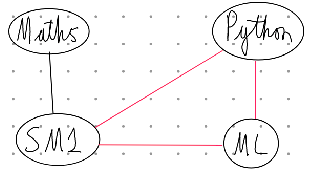
\includegraphics[width=\textwidth/2]{images/factor_graph.png}
    \centering
    \end{figure}
    Where in black is the edges corresponding to the clique given by the first factor and in red the edges corresponding to the clique given by the second factor. The conditional independencies encoded by this graph are:
    \begin{enumerate}
        \item Maths $\bot$ Python $|$ SM1
        \item Maths $\bot$ Python $|$ SM1, ML 
        \item Maths $\bot$ ML $|$ SM1
        \item Maths $\bot$ ML $|$ SM1 , Python
        \item Maths $\bot$ ML, Python $|$ SM1
    \end{enumerate}
    Which are all the conditional independencies of $p(\text{Maths}, \text{SM}1, \text{Python}, \text{ML})$. 

    Now we will create G using all the conditional independencies, which are:
    \begin{enumerate}
        \item Maths $\bot$ Python $|$ SM1
        \item Maths $\bot$ Python $|$ SM1, ML 
        \item Maths $\bot$ ML $|$ SM1
        \item Maths $\bot$ ML $|$ SM1 , Python
        \item Maths $\bot$ ML, Python $|$ SM1
    \end{enumerate}
    The graph we get is the same as before, and reading the graph its clear that it encodes the factorization of $p(\text{Maths}, \text{SM}1, \text{Python}, \text{ML})$. Hence, shown.
\end{question}

\subsection{For Section 2}
\begin{question}
    \textbf{Suppose graph G encodes all conditional independencies in your Gaussian distribution $p(\x)$. Let's say G contains 3 edges and 5 nodes. How many non-zero elements are there in inverse covariance matrix of p?:} \\
    There are 25 entries in $\bm{\Theta}$ and in the adjacency matrix of G (also with 25 entries) there are 6 non-zero (ie. equal to 1) entries hence only 6 entries in $\bm{\Theta}$ that are non-zero (from \cref{equation:adjacency-Theta}). 
\end{question}

\begin{question}\label{question:logistic-regression}
    \textbf{In \cref{subsubsection:Logistic-Regression} we constructed a logistic regression from our simple Markov network model where $\hat{\bm{\beta}}, \hat{\beta_{0}} = \argmax_{\bm{\beta}, \beta_{0}} \sum_{i=1}^{n} \log(p(y_{i}|\xui;\bm{\beta},\beta_{0}))$ show that this is the same logistic regression we talked about in portfolio 3:} \\
    Note that we can write:
    \begin{equation}
        p(y=-1| \x) = 1 / (1+ \frac{p(\x|y=+1)p(y=+1)}{p(\x|y=-1) p(y=-1)})
    \end{equation}
    And for $p(y=-1|\x)$ the same is true but with the inverse of the ratio of the densities. We can rewrite this more generally as:
    \begin{equation}
        p(y | \x; \bm{\beta}, \beta_{0}) = \sigma(f(\x;\bm{\beta}, \beta_{0}) \cdot y)
    \end{equation}
    where $f(\x;\bm{\beta}, \beta_{0}) = log( [p(\x|y=+1)p(y=+1)] / [p(\x|y=-1) p(y=-1)] )$. Hence we can rewrite our MLE as the logistic regression:
    \begin{equation}
        \hat{\bm{\beta}}, \hat{\beta_{0}} = \argmax_{\bm{\beta}, \beta_{0}} \sum_{i=1}^{n} \log (\sigma(f(\xui;\bm{\beta}, \beta_{0}) \cdot y_{i}))
    \end{equation}
    Which is the same logistic regression we had in portfolio 3.
\end{question}


\subsection{For Section 3}
\begin{question}
    \textbf{Given the simple Bayesian Network model described in \cref{section:Bayesian-Network}, however, now with one additional node $X'$ which has one inbound directed edge from $X^{(1)}$. Given this Bayesian Network for a classification task, should you include feature $X'$ for classification? and why?} \\
    To be able to solve the classification problem we would like to find $p(Y|X)$ which for this Bayesian Network is equal to:
    \begin{equation}
        P(Y|X) = \frac{\prod_{i} P(X^{(i)} | Y) P(Y)P(X' | X^{(1)}) }{P(X)}
    \end{equation}
    Hence, we should include feature $X'$ for classification as our factorization and therefore prediction depends on it. 
\end{question}


\end{appendices}
\end{document}